\chapter{EMT Problems}
\section{Magnetostatics}
\begin{enumerate}
	\item  A spherical shell of radius $R$, carrying a uniform surface charge $\sigma$, is set spinning at angular velocity $\omega$. Find its Magnetic dipole moment.
	\begin{answer}
		 The total charge on the shaded ring is
		 \begin{figure}[H]
		 	\centering
		 	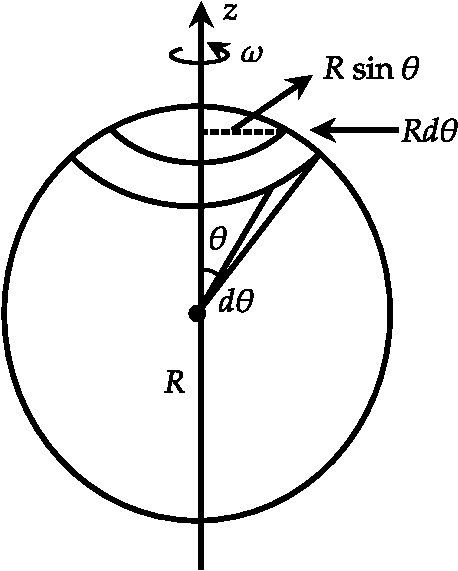
\includegraphics[height=5cm,width=4.5cm]{EM prblm-01}
		 \end{figure}
		\begin{align*}
		d q&=\sigma(2 \pi R \sin \theta) R d \theta\\
	\text{	Time for one revolution is }d t&=\frac{2 \pi}{\omega}\\
		\Rightarrow\text{ Current in the ring }I&=\frac{d q}{d t}=\sigma \omega R^{2} \sin \theta d \theta
		\intertext{Area of the ring $=\pi(\mathrm{R} \sin \theta)^{2}$, so the magnetic moment of the ring is}
		d m&=\left(\sigma \omega R^{2} \sin \theta d \theta\right) \times \pi R^{2} \sin ^{2} \theta\\
		m=\sigma \omega R^{4} \int_{0}^{\pi} \sin ^{3} \theta d \theta&=\frac{4}{3} \pi \times . \sigma \omega R^{4} \Rightarrow \vec{m}=\frac{4 \pi}{3} \sigma \omega R^{4} \hat{z}
		\end{align*}
	\end{answer}
	\item  A solid cylinder of radius $R$ has total charge $Q$ distributed uniformly over its volume and uniform mass density has total mass $M$. It is rotating about its axis with angular speed $\omega$. If its angular momentum is $L$ and magnetic moment is $\mu$, then find the ratio $\frac{\mu}{L} .$
	\begin{answer}
		\begin{align*}
	I=\frac{1}{2} M R^{2}, L&=I \omega=\frac{1}{2} M R^{2} \omega\\
		\text{Magnetic moment due to disc }\mu&=\frac{\pi \sigma \omega R^{4}}{4}\\
		\text{Due to cylinder }d \mu&=\frac{\pi \omega R^{4}}{4}(\rho d z) \quad(\sigma \rightarrow \rho d z)\\
		\mu=\frac{\pi \omega R^{4}}{4} \int_{0}^{L} \frac{Q}{\pi R^{2} L} d z&=\frac{Q \omega R^{2}}{4} \quad \Rightarrow \frac{\mu}{L}=\frac{\underline{Q} \omega R^{2}}{\frac{1}{2} M R^{2} \omega}=\frac{Q}{2 M}
		\end{align*}
	\end{answer}
	\item  A current carrying loop is placed in a uniform magnetic field in four different orientations I, II, III and IV. Arrange them in the decreasing order of potential energy.
	 \begin{tasks}(2)
		\task[\textbf{I.}]\begin{figure}[H]
			\centering
			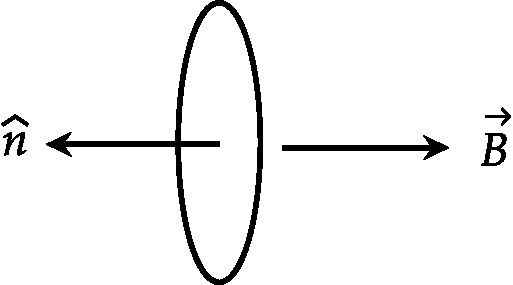
\includegraphics[height=2cm,width=3.5cm]{EM prblm-02}
		\end{figure}
		\task[\textbf{II.}]\begin{figure}[H]
			\centering
			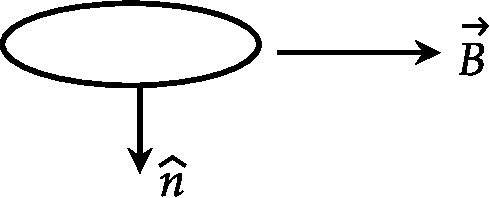
\includegraphics[height=1.5cm,width=3cm]{EM prblm-03}
		\end{figure}
		\task[\textbf{III.}]\begin{figure}[H]
			\centering
			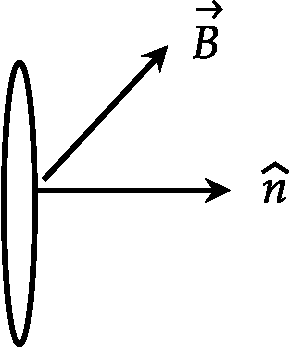
\includegraphics[height=2cm,width=2.5cm]{EM prblm-04}
		\end{figure}
		\task[\textbf{IV.}] \begin{figure}[H]
			\centering
			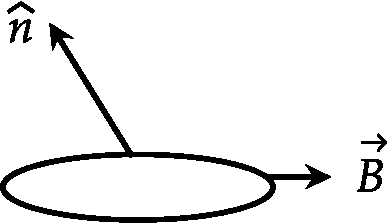
\includegraphics[height=2cm,width=3cm]{EM prblm-05}
		\end{figure}
	\end{tasks}
	\begin{answer}
		\begin{align*}
				\because U&=-\vec{m} \cdot \vec{B}=-m B \cos \theta \\
	\text { I. } \theta=180^{\circ} \Rightarrow U&=+m B, \hspace{1.5cm} \text { II. } \theta=90^{\circ} \Rightarrow U=0 \\
	 \text { III. } \theta=\text { Acute angle } \Rightarrow U&=-v e,  \text { IV. } \hspace{1cm}\theta=\text { Obtuse angle } \Rightarrow U=+v e \\ &\text { Thus } 1>\mathrm{IV}>\mathrm{II}>\mathrm{III} 
		\end{align*}
	\end{answer}
	\item The region between $x=0$ and $x=L$ is filled with uniform, steady magnetic field $B_{0} \hat{k}$. A particle of mass $m$, positive charge $q$ and velocity $v_{0} \hat{i}$ travels along $x$-axis and enters the region of magnetic field. Neglect gravity throughout the question.\\
	(a) Find the value of $L$ if the particle emerges from the region of magnetic field with its final velocity at an angle $30^{\circ}$ to the initial velocity.\\
	(b) Find the final velocity of the particle and the time spent by it in the magnetic field, if the field now extends up to $x=2.1 L$.
	\begin{answer}
		(a) As the initial velocity of the particle is perpendicular to the field the particle will move along the arc of a circle as shown.
		If $r$ is the radius of the circle, then
		\begin{figure}[H]
			\centering
			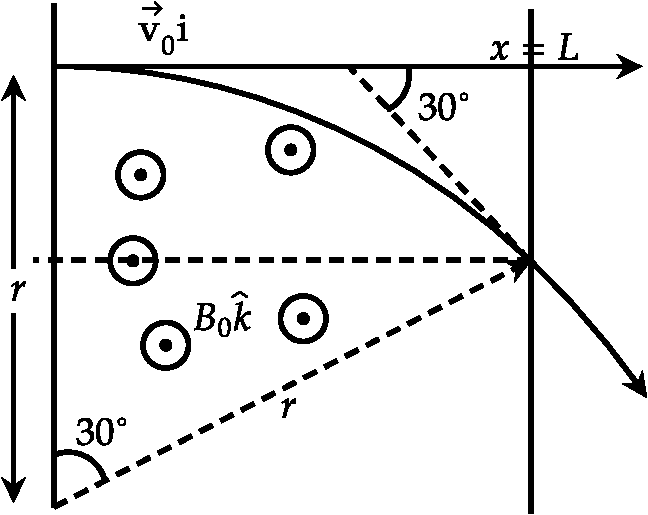
\includegraphics[height=3.7cm,width=5cm]{EM prblm-06}
		\end{figure}
		\begin{align*}
		\frac{m v_{0}^{2}}{r}&=q v_{0} B_{0}\\
		\text{Also from geometry,}\hspace{1cm}
		L&=r \sin 30^{\circ}\\
		\Rightarrow r&=2 L\\
		\text{or}
		L&=\frac{m v_{0}}{2 q B_{0}}\hspace{1cm}\\
	\text{	(b) In this case,}
		L&=\frac{2.1 m v_{0}}{2 q B_{0}}>r
		\end{align*}
		\begin{figure}[H]
			\centering
			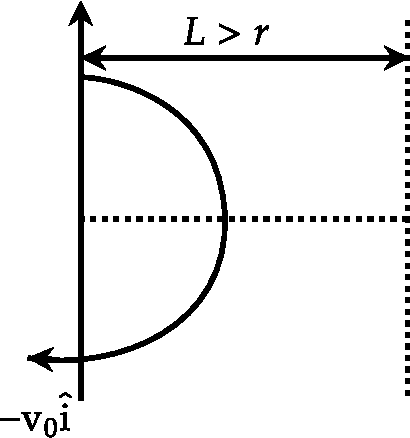
\includegraphics[height=3.5cm,width=3.5cm]{EM prblm-07}
		\end{figure}
			Hence the particle will complete semi-circular path and emerge from the field with velocity $v_{0} \hat{i}$ as shown. Time spent by the particle in the magnetic field
		\begin{align*}
		T=\frac{\pi r}{v_{0}}&=\frac{\pi m}{q B_{0}}
		\end{align*}
		The speed of the particle does not change due to magnetic field.
	\end{answer}
	\item A straight segment $O C$ (of length $L$ meter) of a circuit carrying a current 1 ampere is placed along the $x$-axis. Two infinitely long straight wire $A$ and $B$, each exiuding $z=-\infty$ to $+\infty$ are fixed at $y=-a$ metre and $y=+$ a metre respectively, as shown in the figure. If the wires $A$ and $B$ each carry a current $I$ ampere into the plane of the paper, obtain the cxpression for the force acting on segment $O C$. What will be the force on $O C$ if the current in the wire $B$ is reversed?
	\begin{figure}[H]
		\centering
		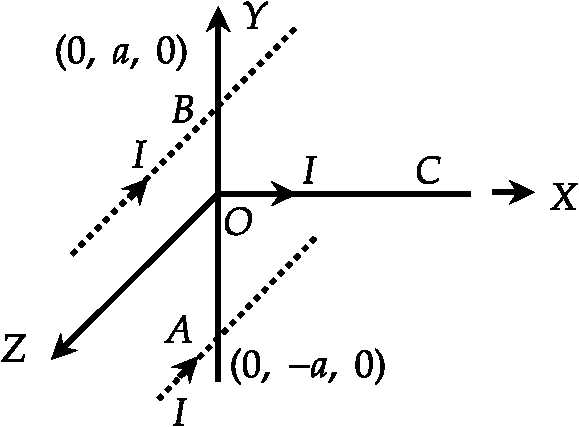
\includegraphics[height=3.2cm,width=5cm]{EM prblm-08}
	\end{figure}
	\begin{answer}
			Magnetic field $B_{A}$ produced at $P(x, 0,0)$ due to wire, $B_{A}=\mu_{0} I / 2 \pi R, B_{B}=\mu_{0} I / 2 \pi R .$ Components of $B_{A}$ and $B_{B}$ along $x$-axis cancel, while those along $y$-axis add up to give total field.
			\begin{figure}[H]
				\centering
				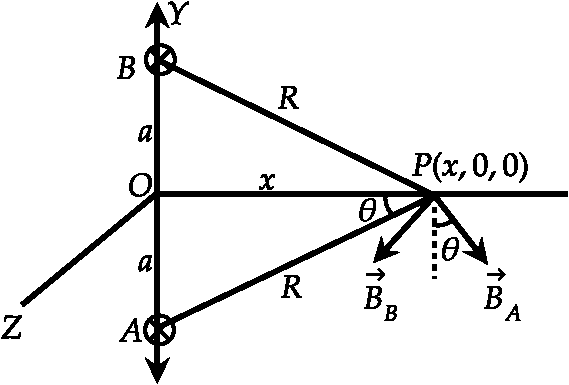
\includegraphics[height=3.5cm,width=5cm]{EM prblm-09}
			\end{figure}
		\begin{align*}
		B&=2\left(\frac{\mu_{0} I}{2 \pi R}\right) \cos \theta=\frac{2 \mu_{0} I}{2 \pi R} \cdot \frac{x}{R}=\frac{\mu_{0} I}{\pi} \frac{x}{\left(a^{2}+x^{2}\right)}\text{ (along $y$ direction)}\\
		\text{The force }&d F\text{ acting on the current element is }d \vec{F}=I(d \vec{l} \times \vec{B})\\
		\therefore \quad d F&=\frac{\mu_{0} I^{2}}{\pi} \frac{x d x}{a^{2}+x^{2}}\hspace{2cm}\left[\because \sin 90^{\circ}=1\right]\\
		\Rightarrow \quad F&=\frac{\mu_{0} I^{2}}{\pi} \int_{0}^{L} \frac{x d x}{a^{2}+x^{2}}=\frac{\mu_{0} I^{2}}{2 \pi} \ln \frac{a^{2}+L^{2}}{a^{2}}
		\end{align*}
		If the current in $B$ is reversed, the magnetic field due to the two wires would be only along $x$-direction and the force on the current along $x$-direction will be zero.
	\end{answer}
\item A wire loop carrying a current $I$ is placed in the $x-y$ plane as shown in figure, (a) If a particle with charge $q$ and mass $m$ is placed at the centre $P$ and given a velocity $v$ along $N P$, find its instantaneous acceleration. (b) If an external uniform magnetic induction $\vec{B}=B \hat{i}$ is applied, find the force and torque acting on the loop.
\begin{answer}
		As in case of current-carrying straight conductor and arc, the magnitude of $B$ is given by
	\begin{align*}
	B_{1}&=\frac{\mu_{0} I}{4 \pi d}(\sin \alpha+\sin \beta) \\
	\text{and}\hspace{1cm}B_{2}&=\frac{\mu_{0} I \phi}{4 \pi r}
	\intertext{So in accordance with right hand screw rule,}
	\end{align*}
	\begin{align*}
	\left(\vec{B}_{w}\right)&=\frac{\mu_{0}}{4 \pi} \frac{1}{(a \cos 60)} \times 2 \sin 60(-\hat{k})\\
	\text{and due to arc}\hspace{1cm}
	(\vec{B})_{M N}&=\frac{\mu_{0}}{4 \pi} \cdot \frac{I}{a} \times\left(\frac{2}{3} \pi\right)(+\hat{k})
\intertext{	and hence net $\vec{B}$ at $P$ due to the given loop}
	\vec{B}&=\vec{B}_{w}+\vec{B}_{A} \\
	\Rightarrow \vec{B}&=\frac{\mu_{0}}{4 \pi} \cdot \frac{2 I}{a}\left[\sqrt{3}-\frac{\pi}{3}\right](-\hat{k})
\intertext{	Now as force on charged particle in a magnetic field is given by}
	\vec{F}&=q(\vec{v} \times \vec{B})\\
\text{	So here,}\hspace{1cm}
	\vec{F}&=q v B \sin 90^{\circ} \text { along } P F \\
	\vec{F}&=\frac{\mu_{0}}{4 \pi} \frac{2 q v}{a}\left[\sqrt{3}-\frac{\pi}{3}\right] \text { along } P F\\
\text{	and so }\quad
	\vec{a}&=\frac{\vec{F}}{m}=10^{-7} \frac{2 q v I}{a}\left[\sqrt{3}-\frac{\pi}{3}\right] \text { along } P F\\
	\text{(b) As }\hspace{1cm}d \vec{F}&=I d \vec{L} \times \vec{B},\text{ so }\vec{F}=\int I d \vec{L} \times \vec{B}\\
\text{	As here $I$ and $\vec{B}$ are constant
	}\quad
	\vec{F}&=I[\oint d \vec{L}] \times \vec{B}=0\quad[\text { as } \oint d \vec{L}=0]\\
	\text{Further as area of coil,}\quad
	\vec{S}&=\left[\frac{1}{3} \pi a^{2}-\frac{1}{2} \cdot 2 a \sin 60^{\circ} \times a \cos 60^{\circ}\right] \hat{k}=a^{2}\left[\frac{\pi}{3}-\frac{\sqrt{3}}{4}\right] \hat{k}\\
\text{	So}\quad
	\vec{M}&=I \vec{S}=I a^{2}\left[\frac{\pi}{3}-\frac{\sqrt{3}}{4}\right] \hat{k}\\
\text{	and hence}\quad
	\vec{\tau}
	&=\vec{M} \times \vec{B}=I a^{2} B\left[\frac{\pi}{3}-\frac{\sqrt{3}}{4}\right](\hat{k} \times \hat{i})\\
	 \text{i.e.}\qquad\vec{\tau}&=I a^{2}\qquad B\left[\frac{\pi}{3}-\frac{\sqrt{3}}{4}\right] \hat{j} N-m
	\quad\operatorname{as}(\hat{k} \times \hat{i}=\hat{j})
	\end{align*}
\end{answer}
	\item 11. A uniform magnetic field of $30 m T$ exists in the $+x$ direction. A particle of charge $+e$ and mass $1.67 \times 10^{-27} \mathrm{~kg}$ is projected into the field along the $+y$ direction with a speed of $4.8 \times 10^{6} \mathrm{~m} / \mathrm{s} .$\\
	(a) Find the force on the charged particle in magnitude and direction.\\
	(b) Find the force if the particle were negatively charged.\\
	(c) Describe the nature of path followed by the particle in both the cases.
	\begin{answer}
			(a) Force acting on a charge particle moving in the magnetic field
		\begin{align*}
	\vec{F}&=q(\vec{v} \times \vec{B})\\
	\text{Magnetic field}
	\vec{B}&=30(m T) \hat{j}\\
\text{	Velocity of the charge particle }\quad \vec{v}&=4.8 \times 10^{6}(\mathrm{~m} / \mathrm{s}) \hat{j}\\
\vec{F}&=1.6 \times 10^{-19}\left[\left(4.8 \times 10^{6} \hat{j}\right) \times\left(30 \times 10^{-3}\right)(\hat{i})\right]\\
\vec{F}&=230.4 \times 10^{-16}(-\hat{k}) N
\intertext{	(b) If the particle were negatively charged, the magnitude of the force will be the same but the direction will be along $(+z)$ direction.}
\intertext{	(c) Since, $\vec{v} \perp \vec{B}$, the path described is a circle}
 R &=\frac{m v}{q B}=\left(1.67 \times 10^{-27}\right) \cdot\left(4.8 \times 10^{6}\right) /\left(1.6 \times 10^{-19}\right) \cdot\left(30 \times 10^{-3}\right) \\ &=1.67 \mathrm{~m} .
		\end{align*}
	\end{answer}
	\item A disc of radius $R$ rotates at an angular velocity $\omega$ about the axis perpendicular to its surface and passing through its centre. If the disc has a uniform surface charge density $\sigma$, find the magnetic induction on the axis of rotation at a distance $x$ from the centre.
	\begin{answer}
		Consider a ring of radius $r$ and width $d r$.
		\begin{align}
		\text{	Charge on the ring,}	d q&=(2 \pi r d r) \sigma\notag\\
	\text{	Current due to ring is }d I&=\frac{d q}{T}\notag\\
	&=\frac{\omega d q}{2 \pi}=\sigma \omega r d r\notag
\intertext{	Magnetic field due to ring at point $P$ is}\notag
	d B&=\frac{\mu_{0} d l r^{2}}{2\left(r^{2}+x^{2}\right)^{3 / 2}}\notag\\
\text{	or}\quad
	B&=\int d B=\frac{\mu_{0} \sigma \omega}{2} \int_{0}^{R} \frac{r^{3} d r}{\left(r^{2}+x^{2}\right)^{3 / 2}}\label{emp20}\\
\text{	Putting }r^{2}+x^{2}=t^{2}\text{ and }2 r d r&=2 t d t\text{ and integrating (\ref{emp20}), we get}\notag\\
	B&=\frac{\mu_{0} \sigma \omega}{2}\left[\frac{R^{2}+2 x^{2}}{\sqrt{R^{2}+x^{2}}}-2 x\right]\notag
		\end{align}
	\end{answer}
	
	
	
	
	
	
	
	
	
	
	
	
	
	
	
	
	
	
	
	
	
\end{enumerate}